\section{Introduction}
First, we will look at the basic mathematical concepts that ultimately underpin the whole theory. So let's start with so-called meshes and look at some examples and how these mathematical concepts can be implemented in code using \maniflow{}.
\begin{defi}[Mesh]
    Let $V$ be a vector space  over $\R$ of dimension $n$. Let $\mathcal{V}_M\subset V$ be a set of points in $V$. We further let $\mathcal{F}_M\subset\mathcal{V}_M^3$. The pair $M = (\mathcal{V}_M, \mathcal{F}_M)$ is then called mesh. The elements of $\mathcal{V}_M$ are called points of $M$ and the elements of $\mathcal{F}_M$ are the faces of the mesh $M$.
\end{defi}
For a mesh $M = (\mathcal{V}_M, \mathcal{F}_M)$ we will often denote $V_M = \vert\mathcal{V}_M\vert$ and $F_M = \vert\mathcal{F}_M\vert$.
\paragraph{Remark.} Meshes $M$ can be considered as $2$-dimensional simplicial complexes. Thus for $2$-dimensional manifolds $\Tilde{M}\subset V$ we may find a \textit{triangulation} simplicial complex $K$ of $\Tilde{M}$. The corresponding mesh will be called \textit{triangulation} mesh of the manifold $\Tilde{M}$.
\begin{ex}[Tetrahedron] Let 
\begin{align*}
    \mathcal{V} = \left\{\left(\sqrt{\frac89},0,-\frac13\right),\left(-\sqrt{\frac29},\sqrt{\frac23},-\frac13\right),\left(-\sqrt{\frac29},-\sqrt{\frac23},-\frac13\right), \left(0,0,1\right)\right\}\subset\R^3
\end{align*}
and $\mathcal{F} = \{f\in2^{\mathcal{V}}:\vert f\vert = 3\}$. The mesh $T = (\mathcal{V},\mathcal{F})$ is the tetrahedron, which is displayed in figure \ref{fig:tetra}.
    \begin{figure}[h]
        \centering
        \includesvg[scale=0.6]{img/tetrahedron.svg}
        \caption{Tetrahedron}
        \label{fig:tetra}
    \end{figure}
This can be implemented using \texttt{maniflow} by using the \texttt{Mesh} class:
\begin{lstlisting}
import numpy as np
import itertools
from maniflow.mesh import Mesh, Face

# computing the four vertices of the tetrahedron
v1 = np.array([np.sqrt(8/9), 0, -1/3])
v2 = np.array([-np.sqrt(2/9), np.sqrt(2/3), -1/3])
v3 = np.array([-np.sqrt(2/9), -np.sqrt(2/3), -1/3])
v4 = np.array([0, 0, 1])

tetra = Mesh()
# setting the vertices as the vertices of the new mesh object
tetra.vertices = [v1, v2, v3, v4]
# now we compute the subsets of all the vertices consiting of three vertices
subsets = set(itertools.combinations(list(range(tetra.v)), 3))
# the faces are then set as the faces of tetra
tetra.faces = [Face(tetra, *list(i)) for i in subsets]
\end{lstlisting}
This way, we obtain the \texttt{Mesh} object \texttt{tetra} which represents a tetrahedron.
\end{ex}
\subsection{\texttt{maniflow.mesh.utils.VertexFunction} -- Creating meshes from parameterisations}
The way we created a mesh of a tetrahedron in the previous example is very static and absolutely not suitable if you want to study more complicated geometries. \maniflow{}, however, provides the option of creating meshes quite easily using parameterisations. For this purpose, \maniflow{} provides the wrapper \texttt{maniflow.mesh.utils.VertexFunction}, which executes a given function on all vertices of the mesh and has the resulting mesh as output.
\begin{ex}
    For the following example, we assume that we have a \texttt{Mesh}-object \code{mesh} and we want to shift this mesh by the vector $\begin{pmatrix}1 & 2 & 3\end{pmatrix}^{\intercal}\in\R^3$. For this we make use of a \texttt{VertexFunction}:
    \begin{lstlisting}
# importing the wrapper from maniflow.mesh.utils
from maniflow.mesh.utils import VertexFunction

# implementing the VertexFuntion 'shift'
@VertexFuntion
def shift(vertex):
    return vertex + np.array([1, 2, 3])


# applying 'shift' to 'mesh'
shifted = shift(mesh)
    \end{lstlisting}
    The resulting \texttt{Mesh}, \code{shifted}, is \code{mesh} shifted by the vector $\begin{pmatrix}1 & 2 & 3\end{pmatrix}^{\intercal}\in\R^3$.
\end{ex}
Another application of this would be the creation of meshes from parameterisations $\psi\colon \R^2\supset D\to\R^3$. Oftentimes, the domain $D$ is a cartesian product of two intervals, so $D = I_1\times I_2$.\footnote{Or to be more precise, \maniflow{} makes it easy to create meshes from parametrisations, where the domain $D$ is homoeomorphic to a square.} For this, \maniflow{} provides the class \texttt{maniflow.mesh.parameterized.Grid}.
\begin{ex}[Moebius strip]
We now turn to an example where we want to create a triangulation of a moebius strip. To this end, we will use the parametrisation
\begin{align*}
    \psi\colon [0, 2\pi]\times [-1,1]\to\R^3,\ (u,v)\mapsto\begin{pmatrix}
        \left(1+\frac{v}{2}\cos{\frac{u}{2}}\right)\cos{u}\\
        \left(1+\frac{v}{2}\cos{\frac{u}{2}}\right)\sin{u}\\
        \frac{v}{2}\sin{\frac{u}{2}}
    \end{pmatrix}.
\end{align*}
In order to discretise the set $[0,2\pi]\times[-1,1]$, we make use of \texttt{maniflow.mesh.parametrized.Grid} in order to create a high resolution lattice. Then we can implement a \texttt{VertexFunction} to capture the parametrisation $\psi$ in code and apply it to our lattice.
\begin{lstlisting}
from maniflow.mesh.parameterized import Grid
from maniflow.mesh.utils import VertexFunction


# implementing the parametrisation 1:1 in code as a VertexFunction
@VertexFunction
def moebius(vertex):
    x = vertex[0]
    y = vertex[1]
    x0 = np.cos(x) * (1 + (y / 2) * np.cos(x / 2))
    x1 = np.sin(x) * (1 + (y / 2) * np.cos(x / 2))
    x2 = (y / 2) * np.sin(x / 2)
    return np.array([x0, x1, x2])


u = Grid((0, 2 * np.pi), (-1, 1), 30, 10)  # create a high resolution grid
moebiusMesh = moebius(u)  # mapping the vertices from the grid according to the parametrisation
coincidingVertices(moebiusMesh) # remove the redundant vertices at the joint after making the moebius band
\end{lstlisting}
With this we obtain the \texttt{Mesh}-object \code{moebiusMesh}. Using \texttt{maniflow.mesh.obj.OBJFile}, we can write this mesh to memory as a \texttt{.obj} file
\begin{lstlisting}
from maniflow.mesh.obj import OBJFile

OBJFile.write(moebiusMesh, "examples/moebius.obj")
\end{lstlisting}
Unsurprisingly, one can then load this file into \href{https://www.blender.org/}{Blender} and create pictures of it etc.\footnote{\maniflow{} comes with its own simple renderer. But if you want to do more elaborated computer graphics, you might consider using some other software to render images.} Figure \ref{fig:moubius_blender} shows a screenshot taken from Blender with the \texttt{.obj} file from \href{https://gitlab.gwdg.de/yangshan.xiang/scientific-computing/-/blob/82c42c864b3e46303b208b78720b8109116c78da/examples/moebius.obj}{\url{examples/moebius.obj}}.
\end{ex}
\begin{figure}[ht]
    \centering
    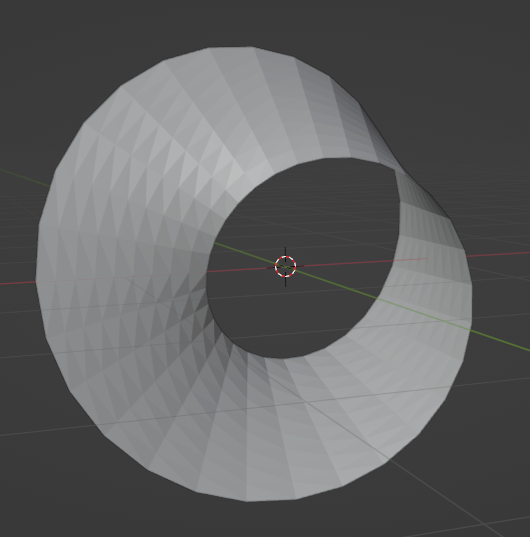
\includegraphics[scale=0.35]{img/moebius_2023-05-23.png}
    \caption{Screenshot of \href{https://www.blender.org/}{Blender} with a moebius strip made with \maniflow{}}
    \label{fig:moubius_blender}
\end{figure}
\section{The face graph of a mesh}
\begin{defi}[Undirected Graph]
    Let $\V_G$ be a set and $\E_G\subset\{e\in2^{\V_G}: |e|=2\}$ be a set of unordered pairs of elements from $\V_G$. The pair $G = (\V_G, \E_G)$ is then called undirected Graph. The elements from $\V_G$ are called vertices of $G$ and the elements from $\E_G$ are called edges of $G$.
\end{defi}
For a Graph $G=(\V_G,\E_G)$ we write
\begin{align*}
    \vcenter{\hbox{\begin{tikzpicture}
    \node (A) at (0,0) {$x$};
    \node (B) at (1,0) {$y$};
    \draw[-] (A) -- (B);\end{tikzpicture}}}
\end{align*}
if $\{x,y\}\in\E_G$. If we take all edges and points together in this way, we get the picture
of a graph with undirected edges.
\begin{ex}
    \begin{equation}\label{eq:sample_g}
    G\colon\left(\vcenter{\hbox{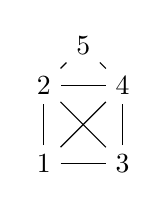
\begin{tikzpicture}[scale=0.5]
    \node (1) at (-1,-1) {$1$};
    \node (2) at (-1,1) {$2$};
    \node (3) at (1,-1) {$3$};
    \node (4) at (1,1) {$4$};
    \node (5) at (0,2) {$5$};
    \draw[-] (1) -- (2);
    \draw[-] (2) -- (3);
    \draw[-] (3) -- (4);
    \draw[-] (4) -- (2);
    \draw[-] (2) -- (5);
    \draw[-] (5) -- (4);
    \draw[-] (4) -- (1);
    \draw[-] (1) -- (3);
\end{tikzpicture}}}\right),\qquad H\colon\left(\vcenter{\hbox{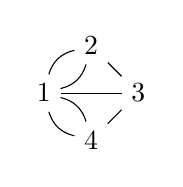
\begin{tikzpicture}[scale=0.6]
\node (1) at (-1, 0) {$1$};
\node (2) at (0, 1) {$2$};
\node (3) at (1,0) {$3$};
\node (4) at (0,-1) {$4$};
\draw[-] (1) -- (3);
\path [-] (1) edge[bend right=-30](2); 
\path [-] (1) edge[bend right=30](2); 
\path [-] (1) edge[bend right=-30](4); 
\path [-] (1) edge[bend right=30](4);
\draw[-] (3) -- (2);
\draw[-] (4) -- (3);
\end{tikzpicture}}}\right)
\end{equation}
\end{ex}
\begin{defi}[Face Graph]
    Let $M = (\mathcal{V}_M, \mathcal{F}_M)$ be a mesh and
    \begin{align*}
        \mathcal{E} = \left\{(f_1,f_2)\in\mathcal{F}_G^2: \vert f_1\cap f_2\vert =2\right\}
    \end{align*}
    The face graph of $M$ is the graph $(\mathcal{F}_M,\mathcal{E})$.
\end{defi}
\begin{ex} The face graph of the tetrahedron is given by
    \begin{equation}\label{eq:sample_g1}
    G\colon\left(\vcenter{\hbox{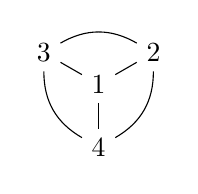
\begin{tikzpicture}[scale=0.8]
    \node (1) at (0,0) {$1$};
    \node (2) at (0.87,0.5) {$2$};
    \node (3) at (-0.87,0.5) {$3$};
    \node (4) at (0,-1) {$4$};
    \draw[-] (1) -- (2);
    \draw[-] (1) -- (3);
    \draw[-] (1) -- (4);
    \path[-] (2) edge[bend right=30] (3);
    \path[-] (3) edge[bend right=30] (4);
    \path[-] (4) edge[bend right=30] (2);
\end{tikzpicture}}}\right)
\end{equation}
\end{ex}
The face graph of a given mesh can be constructed by algorithm \ref{alg:facegraph}.
\begin{algorithm}
    \SetKwInOut{Input}{Input}
    \SetKwInOut{Output}{Output}

    \Input{A mesh $M = (\mathcal{V}_M, \mathcal{F}_M=\{f_1,f_2,f_3\ldots\})$}
    \Output{The adjacency matrix of the face graph of the mesh $M$}
    \caption{Construction of the face graph of a given mesh}
    \label{alg:facegraph}
    $G := 0\in\R^{F_M\times F_M}$\;
    \For{$i=1$ \KwTo $F_M$}
    {
        $neighbors := 0$\;
        \For{$j=1$ \KwTo $F_M$}
        {
            \If{$neighbors = 3$}{
            \textbf{break}\;
            }
            \If{$\vert f_i\cap f_j\vert = 2$ \normalfont{\textbf{and}} $i\neq j$}{
            $G_{ij} \leftarrow 1$\;
            $neighbors \leftarrow neighbors + 1$\;
            }
        }
    }
    \Return{$G$}
\end{algorithm}
Since this algorithm loops over the faces of the mesh in a nested way, the complexity of it lies in $O(F_M^2)$. As this runtime complexity has the consequence of the algorithm being very slow at execution for somewhat large meshes, the face graph is computed dynamically by \texttt{maniflow.mesh.Mesh.faceGraph}.
\subsection{A first application: \texttt{maniflow.mesh.utils.connectedComponents}}
The method \texttt{maniflow.mesh.utils.connectedComponents} decomposes the given mesh into its connected components. Now that we have an algorithm with which to compute the face graph, the connected components of a mesh can now be identified as the connected components of the face graph. These can be determined via the breadth-first traversal of the face graph. 
\begin{algorithm}
    \SetKwInOut{Input}{Input}
    \SetKwInOut{Output}{Output}

    \Input{A mesh $M = (\mathcal{V}_M, \mathcal{F}_M=\{f_1,f_2,f_3\ldots\})$}
    \Output{The connected components of the mesh $M$}
    \caption{Construction of the face graph of a given mesh}
    \label{alg:components}
    Compute the adjacency matrix $G$ using \ref{alg:facegraph}\;
    $start := 1$\;
    $n := 1$\;
    \While{$\mathcal{F}_M\neq\emptyset$}{
        Compute a breadth first traversal sequence $T_n \leftarrow \{f_{start}, f_b,f_c,\ldots\}\subseteq\mathcal{F}_M$\;
        $n \leftarrow n+1$\;
        $\mathcal{F}_M\leftarrow \mathcal{F}_M\setminus T_n$\;
        Set $1< start\leq F_M$ such that $f_{start}\in\mathcal{F}_M$\;
    }
    
    \Return{$T_1$, $T_2$, $\ldots$}
\end{algorithm}
\paragraph{Runtime analysis.} The algorithm \ref{alg:facegraph} has a runtime complexity which lies in $O(F_M^2)$. The breadth-first traversal on the face graph has a runtime\footnote{Since on a graph with the number of vertices being $V$ and the number of edges being $E$ the breadth first search has a complexity of $O(E + V)$. As every face has at most three neighbors we obtain the given runtime complexity.} complexity of $O(F_G + 3\cdot F_G) = O(F_G)$. The computation of $\mathcal{F}_M\setminus T_n$ has also quadratic complexity $O(\vert\mathcal{F}_M\vert^2)$. Thus the overall complexity of algorithm \ref{alg:components} lies in $O(F_G^2)$.
\begin{ex}
    In this example we analyse the connected components of the teapot from \texttt{examples/teapot.obj}. The teapot is displayed in figure \ref{fig:teapot}.
    \begin{figure}[h]
        \centering
        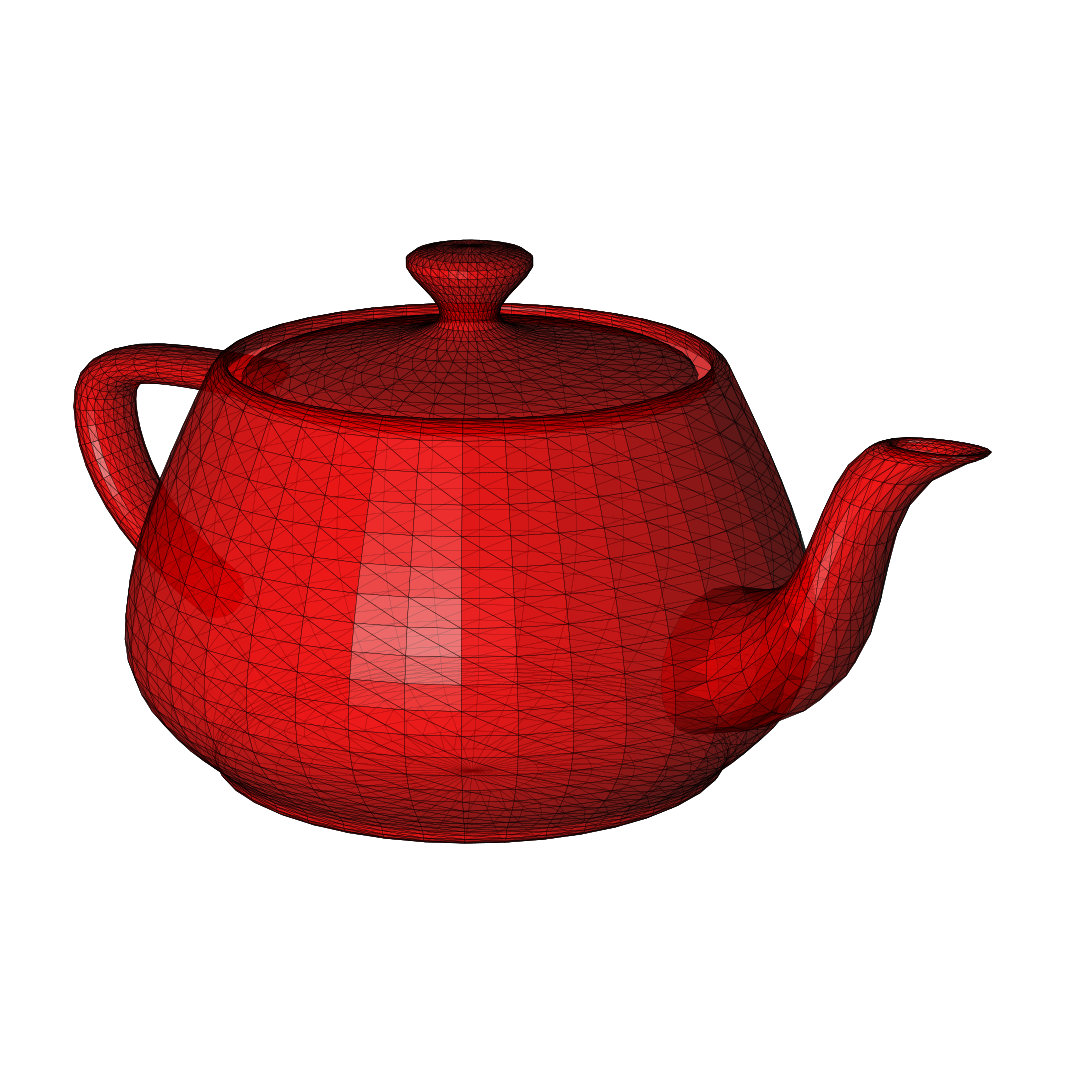
\includegraphics[scale=0.15]{img/teapot.png}
        \caption{The teapot from \texttt{examples/teapot.obj}}
        \label{fig:teapot}
    \end{figure}
    \newline\noindent The connected components can be computed using the following code
    \begin{lstlisting}
from maniflow.mesh import Mesh
from maniflow.mesh.obj import OBJFile
from maniflow.mesh.utils import connectedComponents, coincidingVertices

teapot = OBJFile.read("examples/teapot.obj")
coincidingVertices(teapot)
components = connectedComponents(teapot)

for i, component_list in enumerate(components):
    component = Mesh.fromFaceList(teapot, *component_list)
    OBJFile.write(component, "teapot" + str(i + 1) + ".obj")
    \end{lstlisting}
    \begin{figure}[ht]
    \centering
    \subfloat[The lid of the teapot]{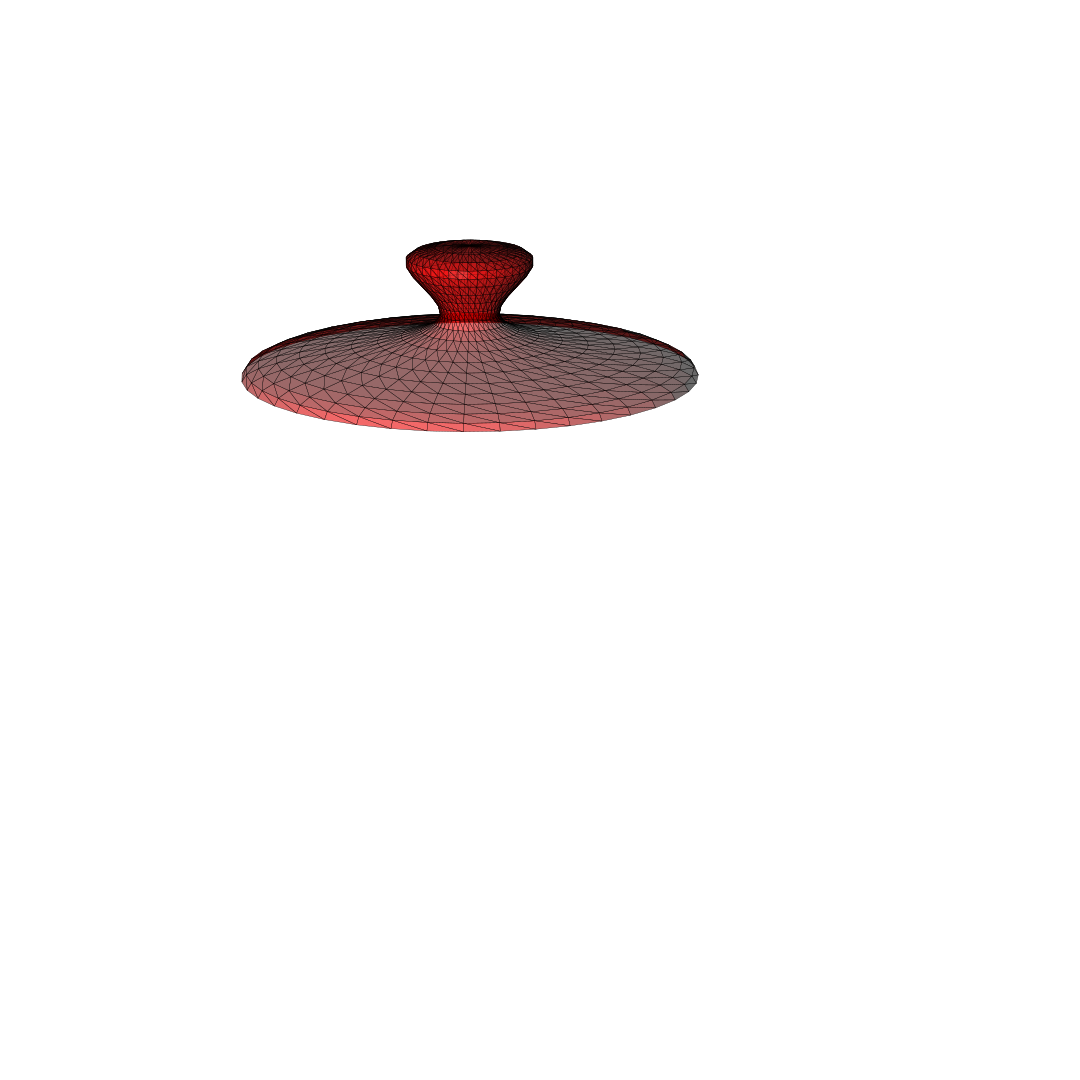
\includegraphics[width=0.4\textwidth]{img/teapot1.png}}\hfil
    \subfloat[The handle of the teapot]{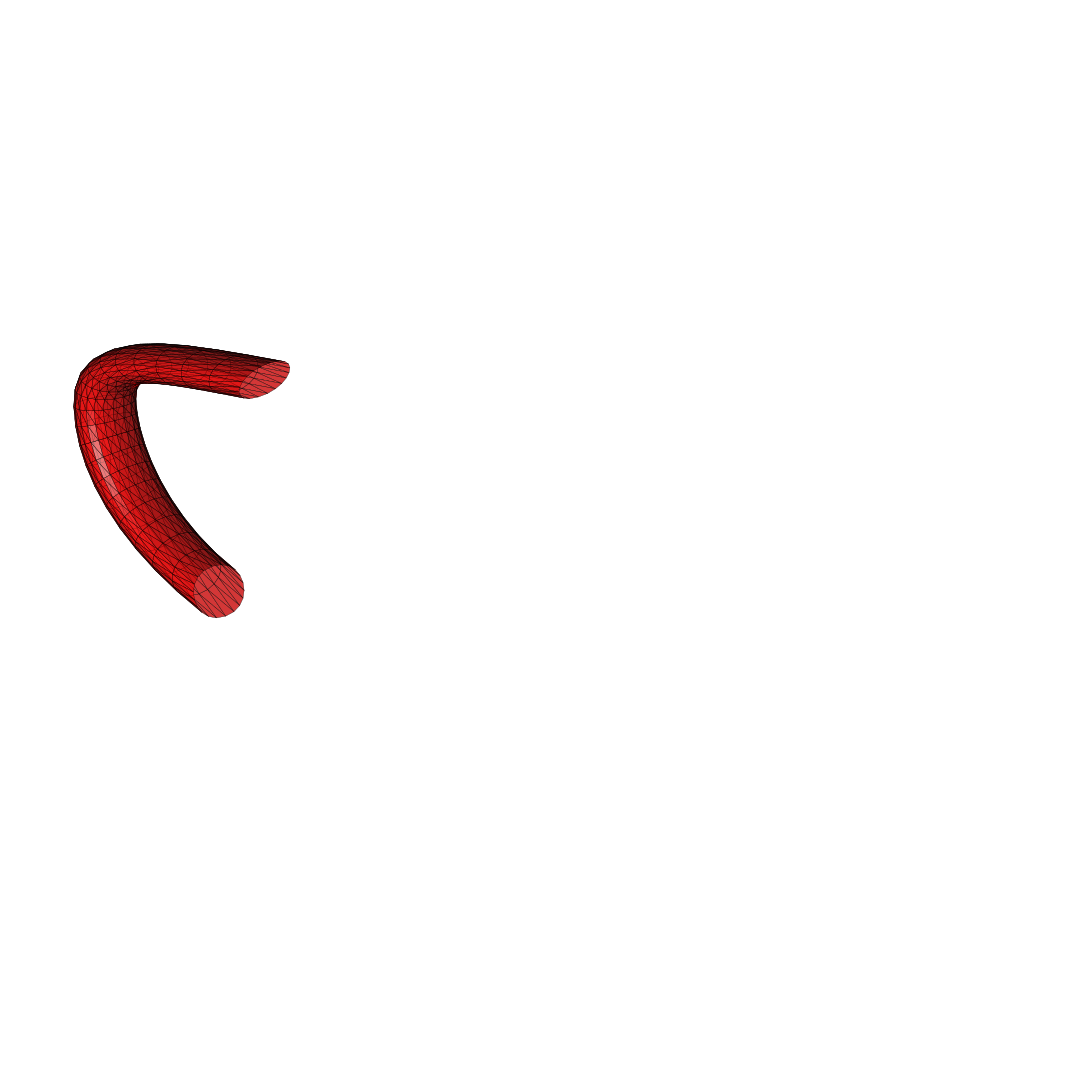
\includegraphics[width=0.4\textwidth]{img/teapot2.png}}\hfil\\
    \subfloat[The body of the teapot]{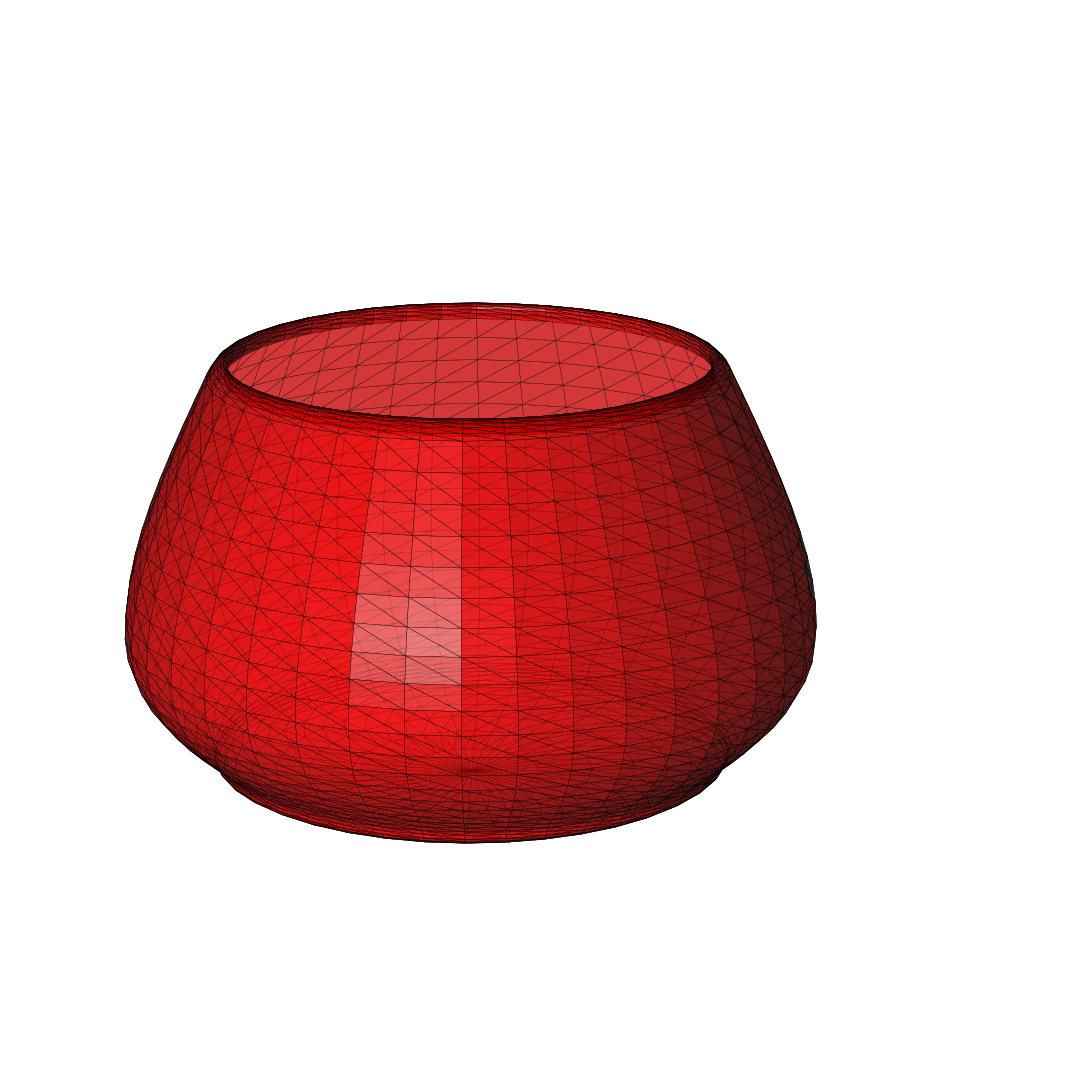
\includegraphics[width=0.4\textwidth]{img/teapot3.png}}\hfil
    \subfloat[The spout of the teapot]{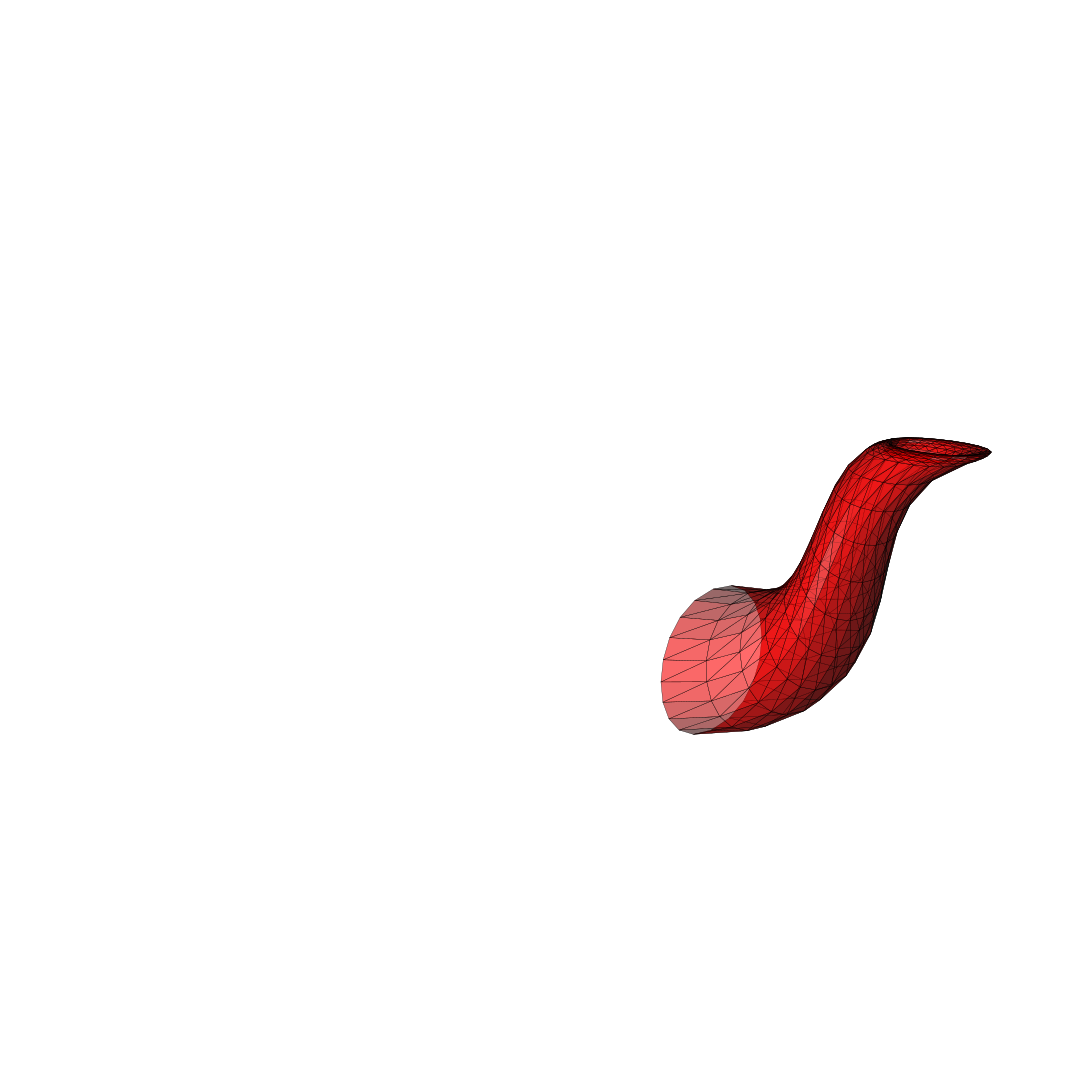
\includegraphics[width=0.4\textwidth]{img/teapot4.png}}\hfil
    \caption{The connected components of the teapot}
    \label{fig:einsteinex}
\end{figure}
\end{ex}
\subsection{Another application: checking orientability of a \texttt{Mesh}}
Orientability of a mesh is equivalent to all vertices being aligned
\begin{figure}
    \centering
    \subfloat[Non compatible orientation]{
    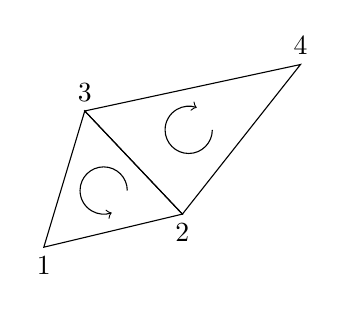
\begin{tikzpicture}
        \draw[]{} (-1.1, -1.13) -- (0.66, -0.71) node[below]{$2$} -- (-0.58, 0.6) node[above]{$3$} -- cycle node[below]{$1$};
        \draw[]{} (0.66, -0.71) -- (-0.58, 0.6) -- (2.16, 1.19) node[above]{$4$} -- cycle;
        \draw[->] (-0.04,-0.41) arc[radius=0.3cm,start angle=0,delta angle=290];
        \draw[->] (1.04,0.36) arc[radius=0.3cm,start angle=0,delta angle=-290];
    \end{tikzpicture}
    }
    \subfloat[Compatible orientation]{
    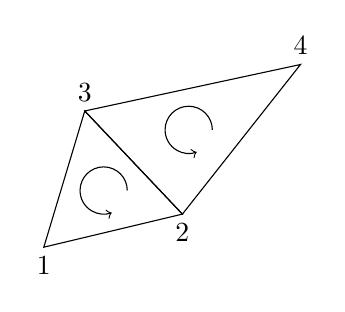
\begin{tikzpicture}
        \draw[]{} (-1.1, -1.13) -- (0.66, -0.71) node[below]{$2$} -- (-0.58, 0.6) node[above]{$3$} -- cycle node[below]{$1$};
        \draw[]{} (0.66, -0.71) -- (-0.58, 0.6) -- (2.16, 1.19) node[above]{$4$} -- cycle;
        \draw[->] (-0.04,-0.41) arc[radius=0.3cm,start angle=0,delta angle=290];
        \draw[->] (1.04,0.36) arc[radius=0.3cm,start angle=0,delta angle=290];
    \end{tikzpicture}
    }
    \caption{Two triangles with compatible and non compatible orientations}
    \label{fig:orientation}
\end{figure}